\chapter{Probabilidade}

\chapter{Probabilidade}

Uma \key{probabilidade} é um número real entre $0$ e $1$
que indica quão provável um evento é.
Se um evento certamente acontecerá,
sua probabilidade é 1,
e se um evento for impossível,
sua probabilidade é 0.
A probabilidade de um evento é denotada por $P(\cdots)$
onde as três reticências descrevem o evento.

Por exemplo, ao lançar um dado,
o resultado é um inteiro entre $1$ e $6$,
e a probabilidade de cada resultado é $1/6$.
Por exemplo, podemos calcular as seguintes probabilidades:

\begin{itemize}[noitemsep]
\item $P(\textrm{''o resultado é 4''})=1/6$
\item $P(\textrm{''o resultado não é 6''})=5/6$
\item $P(\textrm{''o resultado é par''})=1/2$
\end{itemize}

\section{Cálculo}

Para calcular a probabilidade de um evento,
podemos usar a combinatória
ou simular o processo que gera o evento.
Como exemplo, vamos calcular a probabilidade
de tirar três cartas com o mesmo valor
de um baralho de cartas embaralhado
(por exemplo, $\spadesuit 8$, $\clubsuit 8$ e $\diamondsuit 8$).

\subsubsection*{Método 1}

Podemos calcular a probabilidade usando a fórmula

\[\frac{\textrm{número de resultados desejados}}{\textrm{número total de resultados}}.\]

Neste problema, os resultados desejados são aqueles
em que o valor de cada carta é o mesmo.
Existem $13 {4 \choose 3}$ resultados desse tipo,
pois existem $13$ possibilidades para o
valor das cartas e ${4 \choose 3}$ maneiras de
escolher $3$ naipes de $4$ naipes possíveis.

Existem um total de ${52 \choose 3}$ resultados,
pois escolhemos 3 cartas de 52 cartas.
Assim, a probabilidade do evento é

\[\frac{13 {4 \choose 3}}{{52 \choose 3}} = \frac{1}{425}.\]

\subsubsection*{Método 2}

Outra maneira de calcular a probabilidade é
simular o processo que gera o evento.
Neste exemplo, tiramos três cartas, então o processo
consiste em três etapas.
Exigimos que cada etapa do processo seja bem-sucedida.

Tirar a primeira carta certamente será um sucesso,
pois não há restrições.
A segunda etapa é bem-sucedida com probabilidade $3/51$,
pois restam 51 cartas e 3 delas
têm o mesmo valor que a primeira carta.
De forma similar, a terceira etapa é bem-sucedida com probabilidade $2/50$.

A probabilidade de todo o processo ser bem-sucedido é

\[1 \cdot \frac{3}{51} \cdot \frac{2}{50} = \frac{1}{425}.\]

\section{Eventos}

Um evento na teoria da probabilidade pode ser representado como um conjunto
\[A \subset X,\]
onde $X$ contém todos os resultados possíveis
e $A$ é um subconjunto de resultados.
Por exemplo, ao lançar um dado, os resultados são
\[X = \{1,2,3,4,5,6\}.\]
Agora, por exemplo, o evento ''o resultado é par''
corresponde ao conjunto
\[A = \{2,4,6\}.\]

Cada resultado $x$ recebe uma probabilidade $p(x)$.
Então, a probabilidade $P(A)$ de um evento
$A$ pode ser calculada como uma soma
das probabilidades dos resultados usando a fórmula
\[P(A) = \sum_{x \in A} p(x).\]
Por exemplo, ao lançar um dado,
$p(x)=1/6$ para cada resultado $x$,
então a probabilidade do evento
''o resultado é par'' é
\[p(2)+p(4)+p(6)=1/2.\]

A probabilidade total dos resultados em $X$ deve
ser 1, ou seja, $P(X)=1$.

Como os eventos na teoria da probabilidade são conjuntos,
podemos manipulá-los usando operações de conjunto padrão:

\begin{itemize}
\item O \key{complementar} $\bar A$ significa
''$A$ não acontece''.
Por exemplo, ao lançar um dado,
o complementar de $A=\{2,4,6\}$ é
$\bar A = \{1,3,5\}$.
\item A \key{união} $A \cup B$ significa
''$A$ ou $B$ acontecem''.
Por exemplo, a união de
$A=\{2,5\}$
e $B=\{4,5,6\}$ é
$A \cup B = \{2,4,5,6\}$.
\item A \key{interseção} $A \cap B$ significa
''$A$ e $B$ acontecem''.
Por exemplo, a interseção de
$A=\{2,5\}$ e $B=\{4,5,6\}$ é
$A \cap B = \{5\}$.
\end{itemize}

\subsubsection{Complementar}

A probabilidade do complementar
$\bar A$ é calculada usando a fórmula
\[P(\bar A)=1-P(A).\]

Às vezes, podemos resolver um problema facilmente
usando complementares, resolvendo o problema oposto.
Por exemplo, a probabilidade de obter
pelo menos um seis ao lançar um dado dez vezes é
\[1-(5/6)^{10}.\]

Aqui, $5/6$ é a probabilidade de que o resultado
de um único lançamento não seja seis, e
$(5/6)^{10}$ é a probabilidade de que nenhum dos
dez lançamentos seja um seis.
O complementar disso é a resposta para o problema.

\subsubsection{União}

A probabilidade da união $A \cup B$
é calculada usando a fórmula
\[P(A \cup B)=P(A)+P(B)-P(A \cap B).\]
Por exemplo, ao lançar um dado,
a união dos eventos
\[A=\textrm{'''o resultado é par''}\]
e
\[B=\textrm{''o resultado é menor que 4''}\]
é
\[A \cup B=\textrm{''o resultado é par ou menor que 4''},\]
e sua probabilidade é
\[P(A \cup B) = P(A)+P(B)-P(A \cap B)=1/2+1/2-1/6=5/6.\]


Se os eventos $A$ e $B$ são \key{disjuntos}, ou seja,
$A \cap B$ é vazio,
a probabilidade do evento $A \cup B$ é simplesmente

\[P(A \cup B)=P(A)+P(B).\]

\subsubsection{Probabilidade condicional}

\index{probabilidade condicional}

A \key{probabilidade condicional}
\[P(A | B) = \frac{P(A \cap B)}{P(B)}\]
é a probabilidade de $A$
assumindo que $B$ acontece.
Portanto, ao calcular a
probabilidade de $A$, consideramos apenas os resultados
que também pertencem a $B$.

Usando os conjuntos anteriores,
\[P(A | B)= 1/3,\]
pois os resultados de $B$ são
$\{1,2,3\}$, e um deles é par.
Esta é a probabilidade de um resultado par
se sabemos que o resultado está entre $1 \ldots 3$.

\subsubsection{Interseção}

\index{independência}

Usando a probabilidade condicional,
a probabilidade da interseção
$A \cap B$ pode ser calculada usando a fórmula
\[P(A \cap B)=P(A)P(B|A).\]
Os eventos $A$ e $B$ são \key{independentes} se
\[P(A|B)=P(A) \hspace{10px}\textrm{and}\hspace{10px} P(B|A)=P(B),\]
o que significa que o fato de $B$ acontecer não
altera a probabilidade de $A$, e vice-versa.
Neste caso, a probabilidade da interseção é
\[P(A \cap B)=P(A)P(B).\]
Por exemplo, ao tirar uma carta de um baralho, os eventos
\[A = \textrm{''o naipe é paus''}\]
e
\[B = \textrm{''o valor é quatro''}\]
são independentes. Portanto, o evento
\[A \cap B = \textrm{''a carta é o quatro de paus''}\]
acontece com probabilidade
\[P(A \cap B)=P(A)P(B)=1/4 \cdot 1/13 = 1/52.\]

\section{Variáveis aleatórias}

\index{variável aleatória}

Uma \key{variável aleatória} é um valor que é gerado
por um processo aleatório.
Por exemplo, ao lançar dois dados,
uma possível variável aleatória é
\[X=\textrm{''a soma dos resultados''}.\]
Por exemplo, se os resultados forem $[4,6]$
(o que significa que primeiro lançamos um quatro e depois um seis),
então o valor de $X$ é 10.

Denotamos por $P(X=x)$ a probabilidade de que
o valor de uma variável aleatória $X$ seja $x$.
Por exemplo, ao lançar dois dados,
$P(X=10)=3/36$,
pois o número total de resultados é 36
e existem três maneiras possíveis de obter
a soma 10: $[4,6]$, $[5,5]$ e $[6,4]$.

\subsubsection{Valor esperado}

\index{valor esperado}

O \key{valor esperado} $E[X]$ indica o
valor médio de uma variável aleatória $X$.
O valor esperado pode ser calculado como a soma
\[\sum_x P(X=x)x,\]
onde $x$ percorre todos os valores possíveis de $X$.

Por exemplo, ao lançar um dado,
o resultado esperado é
\[1/6 \cdot 1 + 1/6 \cdot 2 + 1/6 \cdot 3 + 1/6 \cdot 4 + 1/6 \cdot 5 + 1/6 \cdot 6 = 7/2.\]

Uma propriedade útil dos valores esperados é a \key{linearidade}.
Isso significa que a soma
$E[X_1+X_2+\cdots+X_n]$
sempre é igual à soma
$E[X_1]+E[X_2]+\cdots+E[X_n]$.
Esta fórmula é válida mesmo se as variáveis aleatórias
dependerem umas das outras.

Por exemplo, ao lançar dois dados,
a soma esperada é
\[E[X_1+X_2]=E[X_1]+E[X_2]=7/2+7/2=7.\]

Vamos agora considerar um problema onde
$n$ bolas são aleatoriamente colocadas em $n$ caixas,
e nossa tarefa é calcular o número esperado
de caixas vazias.
Cada bola tem a mesma probabilidade de
ser colocada em qualquer uma das caixas.
Por exemplo, se $n=2$, as possibilidades
são as seguintes:
\begin{center}
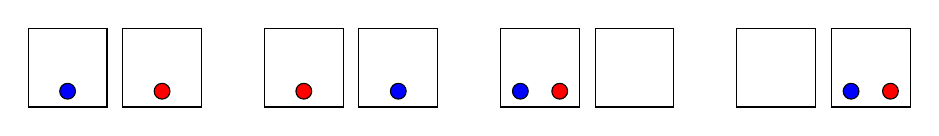
\begin{tikzpicture}
\draw (0,0) rectangle (1,1);
\draw (1.2,0) rectangle (2.2,1);
\draw (3,0) rectangle (4,1);
\draw (4.2,0) rectangle (5.2,1);
\draw (6,0) rectangle (7,1);
\draw (7.2,0) rectangle (8.2,1);
\draw (9,0) rectangle (10,1);
\draw (10.2,0) rectangle (11.2,1);

\draw[fill=blue] (0.5,0.2) circle (0.1);
\draw[fill=red] (1.7,0.2) circle (0.1);
\draw[fill=red] (3.5,0.2) circle (0.1);
\draw[fill=blue] (4.7,0.2) circle (0.1);
\draw[fill=blue] (6.25,0.2) circle (0.1);
\draw[fill=red] (6.75,0.2) circle (0.1);
\draw[fill=blue] (10.45,0.2) circle (0.1);
\draw[fill=red] (10.95,0.2) circle (0.1);
\end{tikzpicture}
\end{center}
Neste caso, o número esperado de
caixas vazias é
\[\frac{0+0+1+1}{4} = \frac{1}{2}.\]
No caso geral, a probabilidade de uma
única caixa estar vazia é
\[\Big(\frac{n-1}{n}\Big)^n,\]
porque nenhuma bola deve ser colocada nela.
Portanto, usando a linearidade, o número esperado de
caixas vazias é
\[n \cdot \Big(\frac{n-1}{n}\Big)^n.\]

\subsubsection{Distribuições}

\index{distribuição}

A \key{distribuição} de uma variável aleatória $X$
mostra a probabilidade de cada valor que
$X$ pode ter.
A distribuição consiste nos valores de $P(X=x)$.
Por exemplo, ao lançar dois dados,
a distribuição da sua soma é:
\begin{center}
\small {
\begin{tabular}{r|rrrrrrrrrrrrr}
$x$ & 2 & 3 & 4 & 5 & 6 & 7 & 8 & 9 & 10 & 11 & 12 \\
$P(X=x)$ & $1/36$ & $2/36$ & $3/36$ & $4/36$ & $5/36$ & $6/36$ & $5/36$ & $4/36$ & $3/36$ & $2/36$ & $1/36$ \\
\end{tabular}
}
\end{center}

\index{distribuição uniforme}
Em uma \key{distribuição uniforme},
a variável aleatória $X$ tem $n$ valores possíveis
$a,a+1,\ldots,b$ e a probabilidade de cada valor é $1/n$.
Por exemplo, ao lançar um dado,
$a=1$, $b=6$ e $P(X=x)=1/6$ para cada valor $x$.

O valor esperado de $X$ em uma distribuição uniforme é
\[E[X] = \frac{a+b}{2}.\]

\index{distribuição binomial}
Em uma \key{distribuição binomial}, $n$ tentativas
são feitas,
e a probabilidade de uma única tentativa ser bem-sucedida
é $p$.
A variável aleatória $X$ conta o número de
tentativas bem-sucedidas,
e a probabilidade de um valor $x$ é
\[P(X=x)=p^x (1-p)^{n-x} {n \choose x},\]
onde $p^x$ e $(1-p)^{n-x}$ correspondem a
tentativas bem-sucedidas e mal-sucedidas,
e ${n \choose x}$ é o número de maneiras
pelas quais podemos escolher a ordem das tentativas.

Por exemplo, ao lançar um dado dez vezes,
a probabilidade de obter um seis exatamente
três vezes é $(1/6)^3 (5/6)^7 {10 \choose 3}$.

O valor esperado de $X$ em uma distribuição binomial é
\[E[X] = pn.\]

\index{distribuição geométrica}
Em uma \key{distribuição geométrica},
a probabilidade de uma tentativa ser bem-sucedida é $p$,
e continuamos até que o primeiro sucesso aconteça.
A variável aleatória $X$ conta o número
de tentativas necessárias, e a probabilidade de
um valor $x$ é
\[P(X=x)=(1-p)^{x-1} p,\]
onde $(1-p)^{x-1}$ corresponde às tentativas malsucedidas
e $p$ corresponde à primeira tentativa bem-sucedida.

Por exemplo, se lançarmos um dado até obtermos um seis,
a probabilidade de que o número de lançamentos
seja exatamente 4 é $(5/6)^3 1/6$.

O valor esperado de $X$ em uma distribuição geométrica é
\[E[X]=\frac{1}{p}.\]

\section{Cadeias de Markov}

\index{cadeia de Markov}

Uma \key{cadeia de Markov}
% \footnote{A. A. Markov (1856--1922)
% foi um matemático russo.}
é um processo aleatório
que consiste em estados e transições entre eles.
Para cada estado, sabemos as probabilidades
de mover para outros estados.
Uma cadeia de Markov pode ser representada como um grafo
cujos nós são estados e arestas são transições.

Como exemplo, considere um problema
em que estamos no andar 1 em um prédio de $n$ andares.
A cada passo, caminhamos aleatoriamente um andar
para cima ou um andar para baixo, exceto que sempre
subimos um andar do andar 1 e descemos um andar
do andar $n$.
Qual é a probabilidade de estar no andar $m$
após $k$ passos?

Neste problema, cada andar do prédio
corresponde a um estado em uma cadeia de Markov.
Por exemplo, se $n=5$, o grafo é o seguinte:

\begin{center}
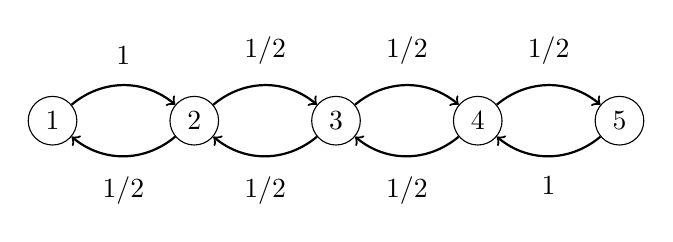
\begin{tikzpicture}[scale=0.9]
\node[draw, circle] (1) at (0,0) {$1$};
\node[draw, circle] (2) at (2,0) {$2$};
\node[draw, circle] (3) at (4,0) {$3$};
\node[draw, circle] (4) at (6,0) {$4$};
\node[draw, circle] (5) at (8,0) {$5$};

\path[draw,thick,->] (1) edge [bend left=40] node[font=\small,label=$1$] {} (2);
\path[draw,thick,->] (2) edge [bend left=40] node[font=\small,label=$1/2$] {} (3);
\path[draw,thick,->] (3) edge [bend left=40] node[font=\small,label=$1/2$] {} (4);
\path[draw,thick,->] (4) edge [bend left=40] node[font=\small,label=$1/2$] {} (5);

\path[draw,thick,->] (5) edge [bend left=40] node[font=\small,label=below:$1$] {} (4);
\path[draw,thick,->] (4) edge [bend left=40] node[font=\small,label=below:$1/2$] {} (3);
\path[draw,thick,->] (3) edge [bend left=40] node[font=\small,label=below:$1/2$] {} (2);
\path[draw,thick,->] (2) edge [bend left=40] node[font=\small,label=below:$1/2$] {} (1);

%\path[draw,thick,->] (1) edge [bend left=40] node[font=\small,label=below:$1$] {} (2);
\end{tikzpicture}
\end{center}

A distribuição de probabilidade
de uma cadeia de Markov é um vetor
$[p_1,p_2,\ldots,p_n]$, onde $p_k$ é a
probabilidade de que o estado atual seja $k$.
A fórmula $p_1+p_2+\cdots+p_n=1$ sempre é válida.

No cenário acima, a distribuição inicial é
$[1,0,0,0,0]$, porque sempre começamos no andar 1.
A próxima distribuição é $[0,1,0,0,0]$,
porque só podemos ir do andar 1 para o andar 2.
Depois disso, podemos subir um andar
ou descer um andar, então a próxima distribuição é
$[1/2,0,1/2,0,0]$, e assim por diante.

Uma maneira eficiente de simular a caminhada em
uma cadeia de Markov é usar programação dinâmica.
A ideia é manter a distribuição de probabilidade,
e a cada passo, percorrer todas as possibilidades
de como podemos nos mover.
Usando este método, podemos simular
uma caminhada de $m$ passos em tempo $O(n^2 m)$.

As transições de uma cadeia de Markov também podem ser
representadas como uma matriz que atualiza a
distribuição de probabilidade.
No cenário acima, a matriz é

\[ 
 \begin{bmatrix}
  0 & 1/2 & 0 & 0 & 0 \\
  1 & 0 & 1/2 & 0 & 0 \\
  0 & 1/2 & 0 & 1/2 & 0 \\
  0 & 0 & 1/2 & 0 & 1 \\
  0 & 0 & 0 & 1/2 & 0 \\
 \end{bmatrix}.
\]

Quando multiplicamos uma distribuição de probabilidade por esta matriz,
obtemos a nova distribuição após mover um passo.
Por exemplo, podemos mover da distribuição
$[1,0,0,0,0]$ para a distribuição
$[0,1,0,0,0]$ da seguinte forma:

\[ 
 \begin{bmatrix}
  0 & 1/2 & 0 & 0 & 0 \\
  1 & 0 & 1/2 & 0 & 0 \\
  0 & 1/2 & 0 & 1/2 & 0 \\
  0 & 0 & 1/2 & 0 & 1 \\
  0 & 0 & 0 & 1/2 & 0 \\
 \end{bmatrix}
 \begin{bmatrix}
  1 \\
  0 \\
  0 \\
  0 \\
  0 \\
 \end{bmatrix}
=
 \begin{bmatrix}
  0 \\
  1 \\
  0 \\
  0 \\
  0 \\
 \end{bmatrix}.
\]

Calculando as potências da matriz de forma eficiente,
podemos calcular a distribuição após $m$ passos
em tempo $O(n^3 \log m)$.

\section{Algoritmos aleatorizados}

\index{algoritmo aleatorizado}

Às vezes, podemos usar a aleatoriedade para resolver um problema,
mesmo que o problema não esteja relacionado a probabilidades.
Um \key{algoritmo aleatorizado} é um algoritmo que
é baseado em aleatoriedade.

\index{algoritmo de Monte Carlo}

Um \key{algoritmo de Monte Carlo} é um algoritmo aleatorizado
que pode, às vezes, dar uma resposta errada.
Para que tal algoritmo seja útil,
a probabilidade de uma resposta errada deve ser pequena.

\index{algoritmo de Las Vegas}

Um \key{algoritmo de Las Vegas} é um algoritmo aleatorizado
que sempre dá a resposta correta,
mas seu tempo de execução varia aleatoriamente.
O objetivo é projetar um algoritmo que seja
eficiente com alta probabilidade.

A seguir, veremos três exemplos de problemas que
podem ser resolvidos usando aleatoriedade.

\subsubsection{Estatísticas de ordem}

\index{estatística de ordem}

A $k$-ésima \key{estatística de ordem} de um array
é o elemento na posição $k$ após a ordenação
do array em ordem crescente.
É fácil calcular qualquer estatística de ordem
em tempo $O(n \log n)$ ordenando primeiro o array,
mas é realmente necessário ordenar o array inteiro
apenas para encontrar um elemento?

Acontece que podemos encontrar estatísticas de ordem
usando um algoritmo aleatorizado sem ordenar o array.
O algoritmo, chamado \key{quickselect}\footnote{Em 1961,
C. A. R. Hoare publicou dois algoritmos que
são eficientes em média: \index{quicksort} \index{quickselect}
\key{quicksort} \cite{hoa61a} para ordenar arrays e
\key{quickselect} \cite{hoa61b} para encontrar estatísticas de ordem.}, é um algoritmo de Las Vegas:
seu tempo de execução é normalmente $O(n)$,
mas $O(n^2)$ no pior caso.

O algoritmo escolhe um elemento aleatório $x$
do array e move os elementos menores que $x$
para a parte esquerda do array,
e todos os outros elementos para a parte direita do array.
Isso leva tempo $O(n)$ quando há $n$ elementos.
Suponha que a parte esquerda contenha $a$ elementos
e a parte direita contenha $b$ elementos.
Se $a=k$, o elemento $x$ é a $k$-ésima estatística de ordem.
Caso contrário, se $a>k$, recursivamente encontramos a $k$-ésima estatística de ordem
para a parte esquerda,
e se $a<k$, recursivamente encontramos a $r$-ésima estatística de ordem
para a parte direita, onde $r=k-a$.
A busca continua de forma similar até que o elemento
tenha sido encontrado.

Quando cada elemento $x$ é escolhido aleatoriamente,
o tamanho do array é dividido pela metade a cada etapa,
então a complexidade de tempo para
encontrar a $k$-ésima estatística de ordem é aproximadamente
\[n+n/2+n/4+n/8+\cdots < 2n = O(n).\]

O pior caso do algoritmo ainda requer tempo $O(n^2)$,
porque é possível que $x$ seja sempre escolhido
de forma que seja um dos menores ou maiores
elementos no array, e $O(n)$ etapas sejam necessárias.
No entanto, a probabilidade disso é tão pequena
que isso nunca acontece na prática.

\subsubsection{Verificação da multiplicação de matrizes}

\index{multiplicação de matrizes}

Nosso próximo problema é \emph{verificar}
se $AB=C$ é válido quando $A$, $B$ e $C$
são matrizes de tamanho $n \times n$.
Claro, podemos resolver o problema
calculando o produto $AB$ novamente
(em tempo $O(n^3)$ usando o algoritmo básico),
mas poderíamos esperar que verificar a
resposta seria mais fácil do que calculá-la do zero.

Acontece que podemos resolver o problema
usando um algoritmo de Monte Carlo\footnote{R. M. Freivalds publicou
este algoritmo em 1977 \cite{fre77}, e às vezes é chamado
de \index{algoritmo de Freivalds} \key{algoritmo de Freivalds}.}, cuja
complexidade de tempo é apenas $O(n^2)$.
A ideia é simples: escolhemos um vetor aleatório
$X$ de $n$ elementos e calculamos as matrizes
$ABX$ e $CX$. Se $ABX=CX$, relatamos que $AB=C$,
caso contrário, relatamos que $AB \neq C$.

A complexidade de tempo do algoritmo é
$O(n^2)$, pois podemos calcular as matrizes
$ABX$ e $CX$ em tempo $O(n^2)$.
Podemos calcular a matriz $ABX$ de forma eficiente
usando a representação $A(BX)$, então apenas duas
multiplicações de matrizes de tamanho $n \times n$ e $n \times 1$
são necessárias.

A desvantagem do algoritmo é
que há uma pequena chance de o algoritmo
cometer um erro ao relatar que $AB=C$.
Por exemplo,
\[
 \begin{bmatrix}
  6 & 8 \\
  1 & 3 \\
 \end{bmatrix}
\neq
 \begin{bmatrix}
  8 & 7 \\
  3 & 2 \\
 \end{bmatrix},
\]
mas
\[
 \begin{bmatrix}
  6 & 8 \\
  1 & 3 \\
 \end{bmatrix}
 \begin{bmatrix}
  3 \\
  6 \\
 \end{bmatrix}
=
 \begin{bmatrix}
  8 & 7 \\
  3 & 2 \\
 \end{bmatrix}
 \begin{bmatrix}
  3 \\
  6 \\
 \end{bmatrix}.
\]
No entanto, na prática, a probabilidade de o
algoritmo cometer um erro é pequena,
e podemos diminuir a probabilidade
verificando o resultado usando vários vetores aleatórios $X$
antes de relatar que $AB=C$.

\subsubsection{Coloração de grafos}

\index{coloração}

Dado um grafo que contém $n$ vértices e $m$ arestas,
nossa tarefa é encontrar uma maneira de colorir os vértices
do grafo usando duas cores, de modo que
para pelo menos $m/2$ arestas, os vértices adjacentes
tenham cores diferentes.
Por exemplo, no grafo
\begin{center}
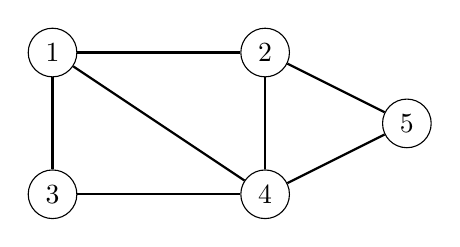
\begin{tikzpicture}[scale=0.9]
\node[draw, circle] (1) at (1,3) {$1$};
\node[draw, circle] (2) at (4,3) {$2$};
\node[draw, circle] (3) at (1,1) {$3$};
\node[draw, circle] (4) at (4,1) {$4$};
\node[draw, circle] (5) at (6,2) {$5$};

\path[draw,thick,-] (1) -- (2);
\path[draw,thick,-] (1) -- (3);
\path[draw,thick,-] (1) -- (4);
\path[draw,thick,-] (3) -- (4);
\path[draw,thick,-] (2) -- (4);
\path[draw,thick,-] (2) -- (5);
\path[draw,thick,-] (4) -- (5);
\end{tikzpicture}
\end{center}
uma coloração válida é a seguinte:
\begin{center}
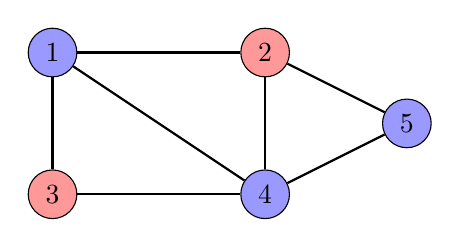
\begin{tikzpicture}[scale=0.9]
\node[draw, circle, fill=blue!40] (1) at (1,3) {$1$};
\node[draw, circle, fill=red!40] (2) at (4,3) {$2$};
\node[draw, circle, fill=red!40] (3) at (1,1) {$3$};
\node[draw, circle, fill=blue!40] (4) at (4,1) {$4$};
\node[draw, circle, fill=blue!40] (5) at (6,2) {$5$};

\path[draw,thick,-] (1) -- (2);
\path[draw,thick,-] (1) -- (3);
\path[draw,thick,-] (1) -- (4);
\path[draw,thick,-] (3) -- (4);
\path[draw,thick,-] (2) -- (4);
\path[draw,thick,-] (2) -- (5);
\path[draw,thick,-] (4) -- (5);
\end{tikzpicture}
\end{center}
O grafo acima contém 7 arestas e, para 5 delas,
os vértices adjacentes têm cores diferentes,
portanto a coloração é válida.

O problema pode ser resolvido usando um algoritmo de Las Vegas
que gera colorações aleatórias até que uma coloração válida
seja encontrada.
Em uma coloração aleatória, a cor de cada vértice é
escolhida independentemente de forma que a probabilidade de receber
qualquer uma das duas cores seja $1/2$.

Em uma coloração aleatória, a probabilidade de os vértices adjacentes
de uma única aresta terem cores diferentes é $1/2$.
Portanto, o número esperado de arestas cujos vértices adjacentes
têm cores diferentes é $m/2$.
Como espera-se que uma coloração aleatória seja válida,
encontraremos rapidamente uma coloração válida na prática.

